\documentclass{article}

\usepackage{graphicx}
\usepackage{tikz}
\usepackage{tikzsymbols}
\usetikzlibrary{calc,patterns,shapes.geometric}
\pagestyle{empty}
\usepackage[margin=0pt]{geometry}
\geometry{papersize={14in,12in}}

\def\centerarc[#1](#2)(#3:#4:#5){\draw[#1] ($(#2)+({#5*cos(#3)},{#5*sin(#3)})$) arc (#3:#4:#5);}

\begin{document}
	\begin{figure}
		\centering
		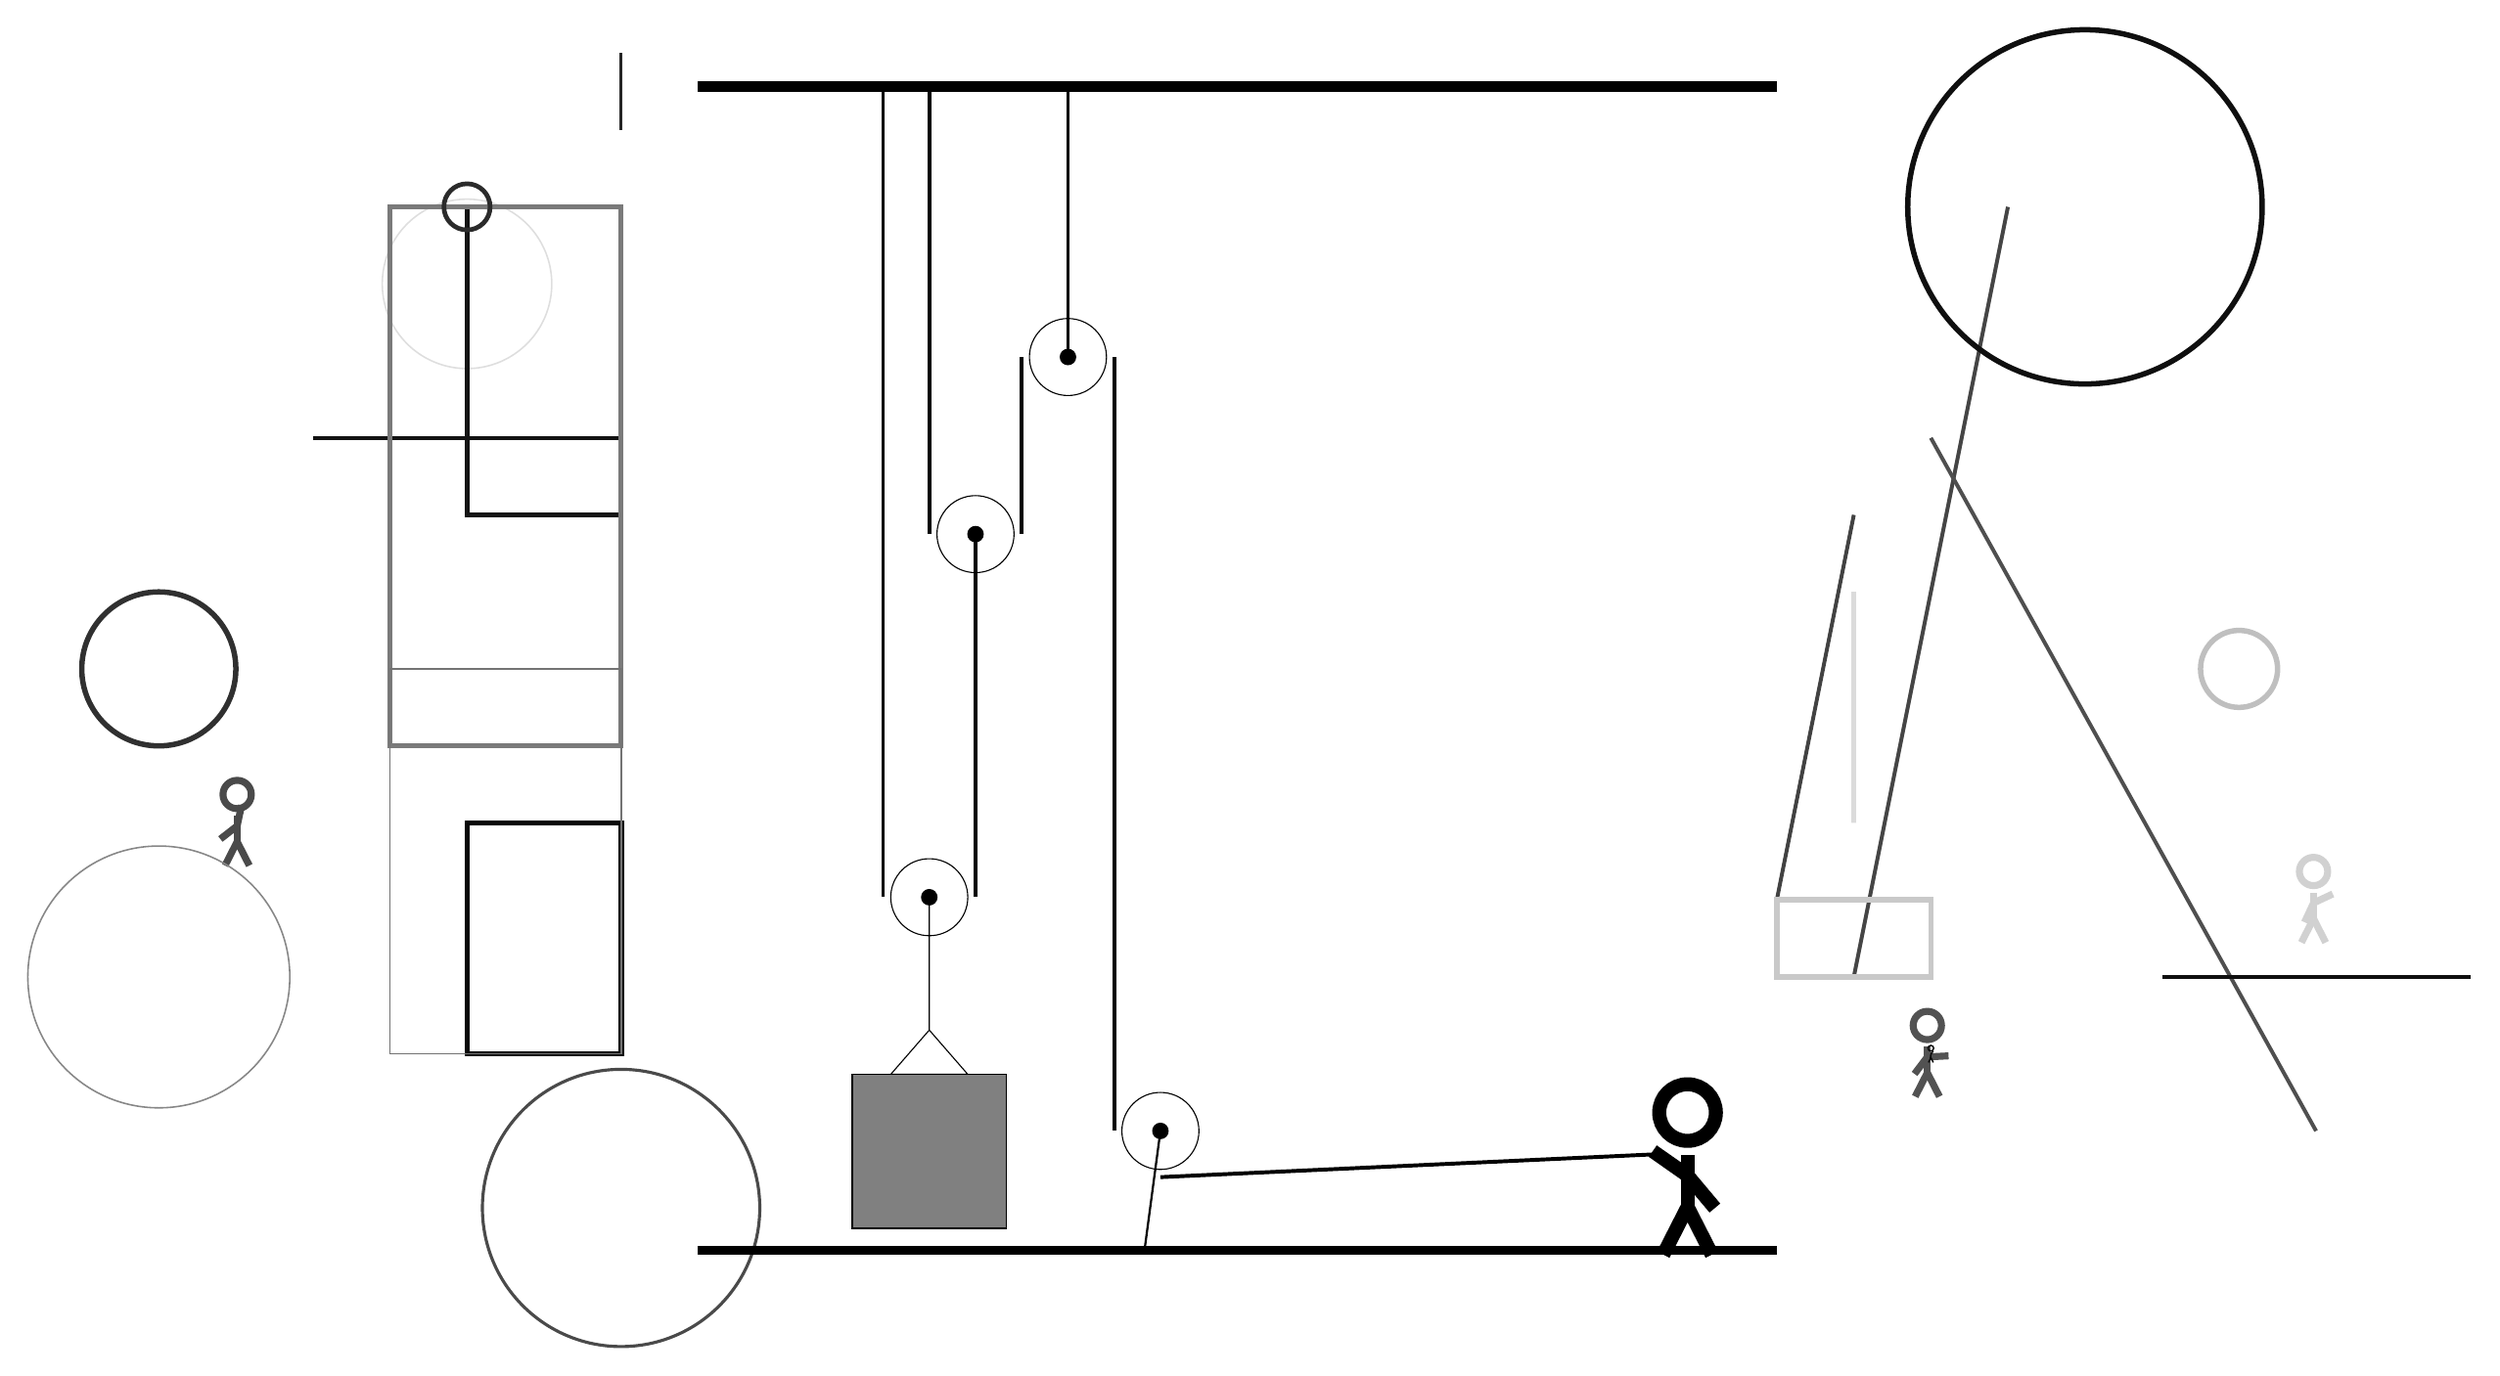
\begin{tikzpicture}
			%%%%% START %%%%%
			
			\draw[fill=black] (-2, 11.5) rectangle (12, 11.625);
			
			\draw (1, 1.035) circle (0.5);
			\draw[fill=black] (1, 1.035) circle (0.1);
			
			\draw (1.6, 5.75) circle (0.5);
			\draw[fill=black] (1.6, 5.75) circle (0.1);
			
			\draw (2.8, 8.05) circle (0.5);
			\draw[fill=black] (2.8, 8.05) circle (0.1);
			\draw[thick] (2.8, 8.05) -- (2.8, 11.5);
			
			\draw (4.0, -2) circle (0.5);
			\draw[fill=black] (4.0, -2) circle (0.1);
			\draw[thick] (4.0, -2) -- (3.8, -3.5);
			
			\draw (1, 1.035) -- (1, -0.69) -- (0.5, -1.265) -- (1.5, -1.265) -- (1, -0.69);
			\draw[fill=black!50] (0, -1.265) rectangle (2, -3.265);
			\draw[line width=0.5mm] (0.4, 11.5) -- (0.4, 1.035);
			\centerarc[line width=0.5mm](1, 1.035)(180:360:0.6);
			\draw[line width=0.5mm](1.6, 1.035) -- (1.6, 5.75);
			\draw[line width=0.5mm] (1.0, 11.5) -- (1.0, 5.75);
			\centerarc[line width=0.5mm](1.6, 5.75)(180:360:0.6);
			\draw[line width=0.5mm](2.2, 5.75) -- (2.2, 8.05);
			\centerarc[line width=0.5mm](2.8, 8.05)(0:180:0.6);
			\draw[line width=0.5mm] (3.4, 8.05) -- (3.4, -2);
			\centerarc[line width=0.5mm](4.0, -2)(0:90:-0.6);
			\draw[line width=0.5mm](4.0, -2.6) -- (10.5, -2.3);
			
			\node at (10.8, -2.5) {\Strichmaxerl[10][-35][-50]};
			
			\draw[line width=0.5mm, color=black!73](13, 0) -- (15, 10);
			
			\draw[line width=0.7mm, color=black!97] (-3, -1) rectangle (-5, 2);
			\node[line width=0.5mm, color=black!18] at (19, 1) {\Strichmaxerl[5][65][25]};
			\draw [line width=0.2mm, color=black!13](-5, 9) circle (1.1);
			
			\node[line width=0.2mm, color=black!68] at (14, -1) {\Strichmaxerl[5][53][3]};
			
			\draw [line width=0.7mm, color=black!81](-9, 4) circle (1.0);
			\draw[line width=0.6mm, color=black!92] (-3, 6) rectangle (-5, 10);
			\draw[line width=0.6mm, color=black!14] (13, 5) rectangle (13, 2);
			\draw [line width=0.7mm, color=black!25](18, 4) circle (0.5);
			\node[line width=0.7mm, color=black!71] at (-8, 2) {\Strichmaxerl[5][38][78]};
			\node[line width=0.4mm, color=black!97] at (14, -1) {\Strichmaxerl[1][83][57]};
			
			\draw [line width=0.7mm, color=black!94](16, 10) circle (2.3);
			\draw[line width=0.4mm, color=black!85] (-3, 11) rectangle (-3, 12);
			
			\draw [line width=0.4mm, color=black!71](-3, -3) circle (1.8);
			\draw[line width=0.5mm, color=black!93](-3, 7) -- (-7, 7);
			\draw[line width=0.5mm, color=black!74](13, 6) -- (12, 1);
			
			\draw[line width=0.7mm, color=black!21] (12, 0) rectangle (14, 1);
			\draw[line width=0.5mm, color=black!69](14, 7) -- (19, -2);
			\draw[line width=0.6mm, color=black!52] (-3, 10) rectangle (-6, 3);
			
			\draw [line width=0.6mm, color=black!83](-5, 10) circle (0.3);
			\draw[line width=0.2mm, color=black!55] (-3, -1) rectangle (-6, 4);
			\draw [line width=0.2mm, color=black!47](-9, 0) circle (1.7);
			\draw[line width=0.5mm, color=black!94](17, 0) -- (21, 0);
			
			\draw[fill=black] (-2, -3.5) rectangle (12, -3.6);
			
			%%%%% END %%%%%
		\end{tikzpicture}
	\end{figure}	
\end{document}